%!TEX root = ../master.tex
\section{Cryptography}
This section will briefly introduce concepts from cryptography relevant to the project, and will be based on \cite{cryptoenginering}.

\subsection{Encryption}
\bruno{Vil vi have det her med? \#62}

\subsection{Authentication}
When Alice sends messages to Bob over some insecure channel it can be possible for Eve to change how Bob receives the messages.
Eve can alter the sent message \emph{m} to \emph{m'} and send \emph{m'} to Bob without Bob knowing.
Eve can also change the order of messages so a message comes much later than intended.
If Eve deletes a message Bob will never know that this message existed.
Eve can even create her own message and send it without Bob can know that this message was not created by Alice.

\begin{figure}[H]
	\centering
	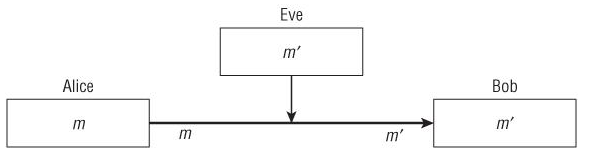
\includegraphics[width=0.6\textwidth]{authenticationNoAuth}
	\caption{The basic problem, who sent \emph{m'}? From \citet[p.~52]{cryptoenginering}}
	\label{crypto:noauth}
\end{figure}

The solution to these problems is authentication of messages \citet[p.~52]{cryptoenginering}.
Alice and Bob have a shared secret key $K_a$ for authentication.
When sending message \emph{m} Alice first computes a Message Authentication Code (MAC).
This authentication code \emph{a} is calculated as $a := h(K_a,m)$, where $h()$ is the MAC function.
Alice now sends both the MAC \emph{a} and the message \emph{m} to Bob.
When Bob receives \emph{a} and \emph{m} he computes the MAC of \emph{m} and compares with the \emph{a} he received from Alice.
The situation is outlined on \cref{crypto:authsetup}

\begin{figure}[H]
	\centering
	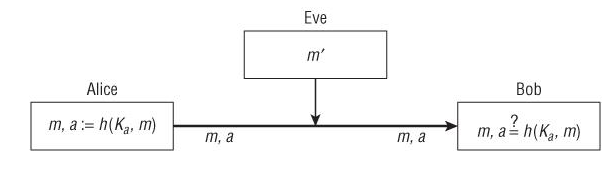
\includegraphics[width=0.6\textwidth]{authenticationSetup}
	\caption{Setup for authentication. From \citet[p.~53]{cryptoenginering}}
	\label{crypto:authsetup}
\end{figure}

If Eve wants to modify the message \emph{m} to the different message \emph{m'} and simply replaces \emph{m} with \emph{m'}, Bob will be able to tell when computing the MAC of \emph{m'}.
This is the case because of the design of the MAC function.
A MAC function is designed such that two different messages \emph{m} and \emph{m'} will not result in the same MAC.
Bob will therefore discard message \emph{m} as an attacked message.

Even with this countermeasure Eve will be able to record a message and MAC pair and send it to Bob at a later point in time.
She can also still delete messages without Bob knowing that it ever existed.
Because of these flaws authentication is almost always accompanied by a numbering scheme which makes it possible for Bob to determine if there is being tampered with the message order.
Eve will still be able to entirely stop the communication between Alice and Bob, or delay it.

\stefan{noget om public key og digitale signaturer?}
